\section{QRコード}
自動車メーカーのデンソーに発明された.
汚れによる耐障害性が非常に高く,非対称なので,向きの検出も可能.
英数字で最大4296文字まで記録が可能

\begin{figure}[htbp]
    \begin{center}
        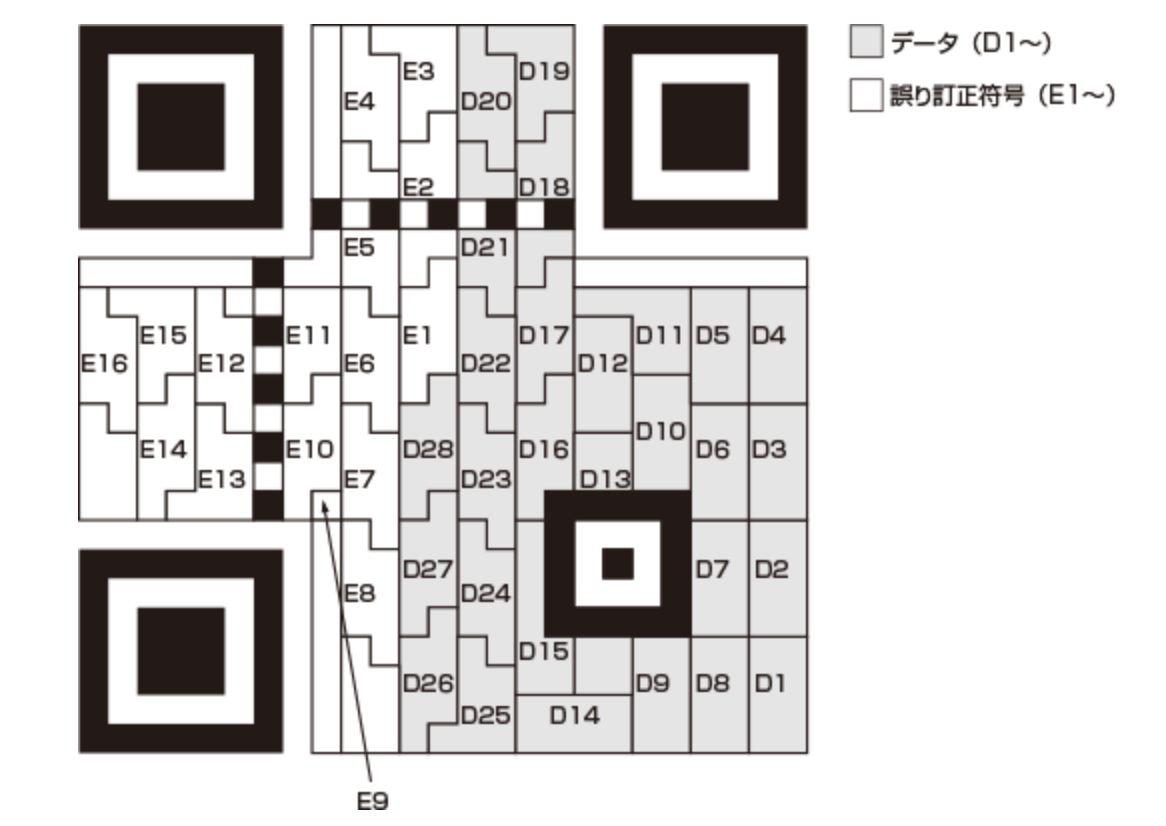
\includegraphics[clip,width=7.0cm]{img/qrcode.png}
        \caption{QRコードの仕様\cite{qrcode}}
    \end{center}
\end{figure}

コンピュータ上で検出する際は以下の手順で検出を行う.
\begin{enumerate}
    \item 水平方向に探索をし,白黒の比が1:1:3:1:1になる箇所を探索しファインパターンの候補として記録する.
    \item 垂直方向に探索をし,ファイパターン候補の中心から上下にそれぞれ白黒の比が3:2:2になるか検証する.
    \item 3箇所のファインパターンが求まれば3点で構成される平行四辺形の頂点から残りの1点を推定し四角を推定します.
\end{enumerate}

データ部分のデコードは右下から順に黒を1白を0として右下のマスを基点として左隣のマス,上のマス,左上のマス,と順に読み取っていく.